% =================================================================================================
% File:			dettaglio_delle_verifiche_tramite_analisi.tex
% Description:	Definisce le verifiche effettuate tramite analisi
% Created:		2014/03/05
% Author:		Faccin Nicola
% Email:		faccin.nicola@mashup-unipd.it
% =================================================================================================
% Modification History:
% Version		Modifier Date		Change											Author
% 0.0.1 		2014/01/11 			iniziata stesura appendice					Lorenzo C.
% =================================================================================================
% Version		Modifier Date		Change											Author
% 1.0.1 		2015/03/17 			iniziata stesura appendice B				Nicola F.
% =================================================================================================
% Version		Modifier Date		Change											Author
% 1.0.2 		2015/03/23			stesura fase 1								Nicola F.
% =================================================================================================
% Version		Modifier Date		Change											Author
% 1.0.3 		2015/03/24 			stesura fase 2								Nicola F.
% =================================================================================================
% Version		Modifier Date		Change											Author
% 1.0.4 		2015/03/25 			stesura fase 3								Nicola F.
% =================================================================================================
% Version		Modifier Date		Change											Author
% 2.0.1 		2015/05/20 			stesura fase 4								Nicola F.
% =================================================================================================
% Version		Modifier Date		Change											Author
% 2.0.2 		2015/05/20 			stesura fase 6								Nicola F.
% =================================================================================================
%

% CONTENUTO DEL CAPITOLO

\section{Dettaglio delle verifiche tramite analisi}
	\subsection{Ricerca ed implementazione degli strumenti}
		\subsubsection{Processi}
		Il seguente grafico deriva dall'analisi dei ticket pianificati, svolti, approvati e verificati dal gruppo in relazione alle date in cui hanno cambiato stato. \\ \\
		Come si può notare in figura 3, c'è una rapida crescita di task pianificati nelle date dei verbali interni che corrispondono alle riunioni del gruppo, nonché ai verbali interni. Verso la fine della fase si osserva un aumento dei task approvati e verificati, questo per tentare di completare tutti quelli pianificati entro la data di fine fase. Si nota in oltre che non tutti i task sono stati completati entro la fine della fase, questo andrà ad appesantire dunque la fase successiva che si verrà a trovare i task della fase precedente da completare.
			\begin{figure}[htbp]
				\centering
				\centerline{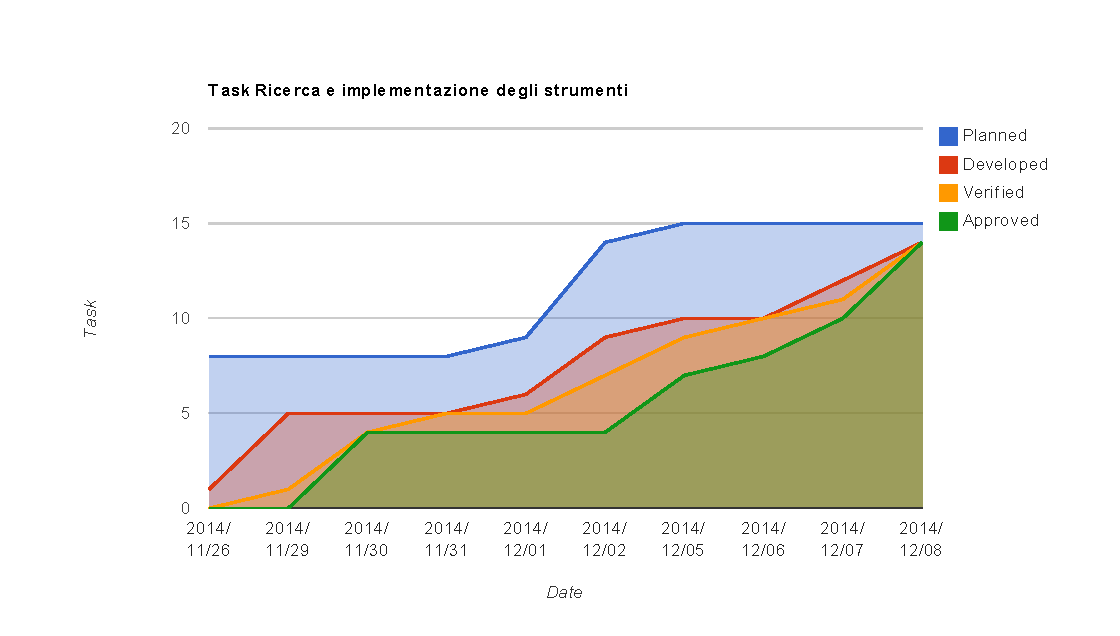
\includegraphics[scale=1]{images/Grafico_fase_1.pdf}}
				\caption{Grafico task Ricerca ed implementazione degli strumenti}
				\label{fig:taskfase1}
			\end{figure}
		\subsubsection{Documenti}
		Essendo in questa fase non presente ancora alcun documento, non è stato possibile verificarli e quindi avere dei valori da esporre. Per correttezza è stato comunque inserito il nome della fase.
	
	\subsection{Analisi dei requisiti}
		\subsubsection{Processi}
		La figura 4 rappresenta l'andamento dei task relativi a questa fase, si nota che dato l'inesperienza del gruppo e il tipo di fase in cui ci troviamo, inizialmente non ci sono molti task pianificati come ci si potrebbe aspettare in altre fasi. Il gruppo ha proseguito a pianificare pochi task alla volta fino al primo incontro con il proponente. Dal 2015/01/14 si osserva infatti un notevole picco inizialmente per i Planned ma poi anche per i Developed Verified e Approved. 
			\begin{figure}[htbp]
				\centering
				\centerline{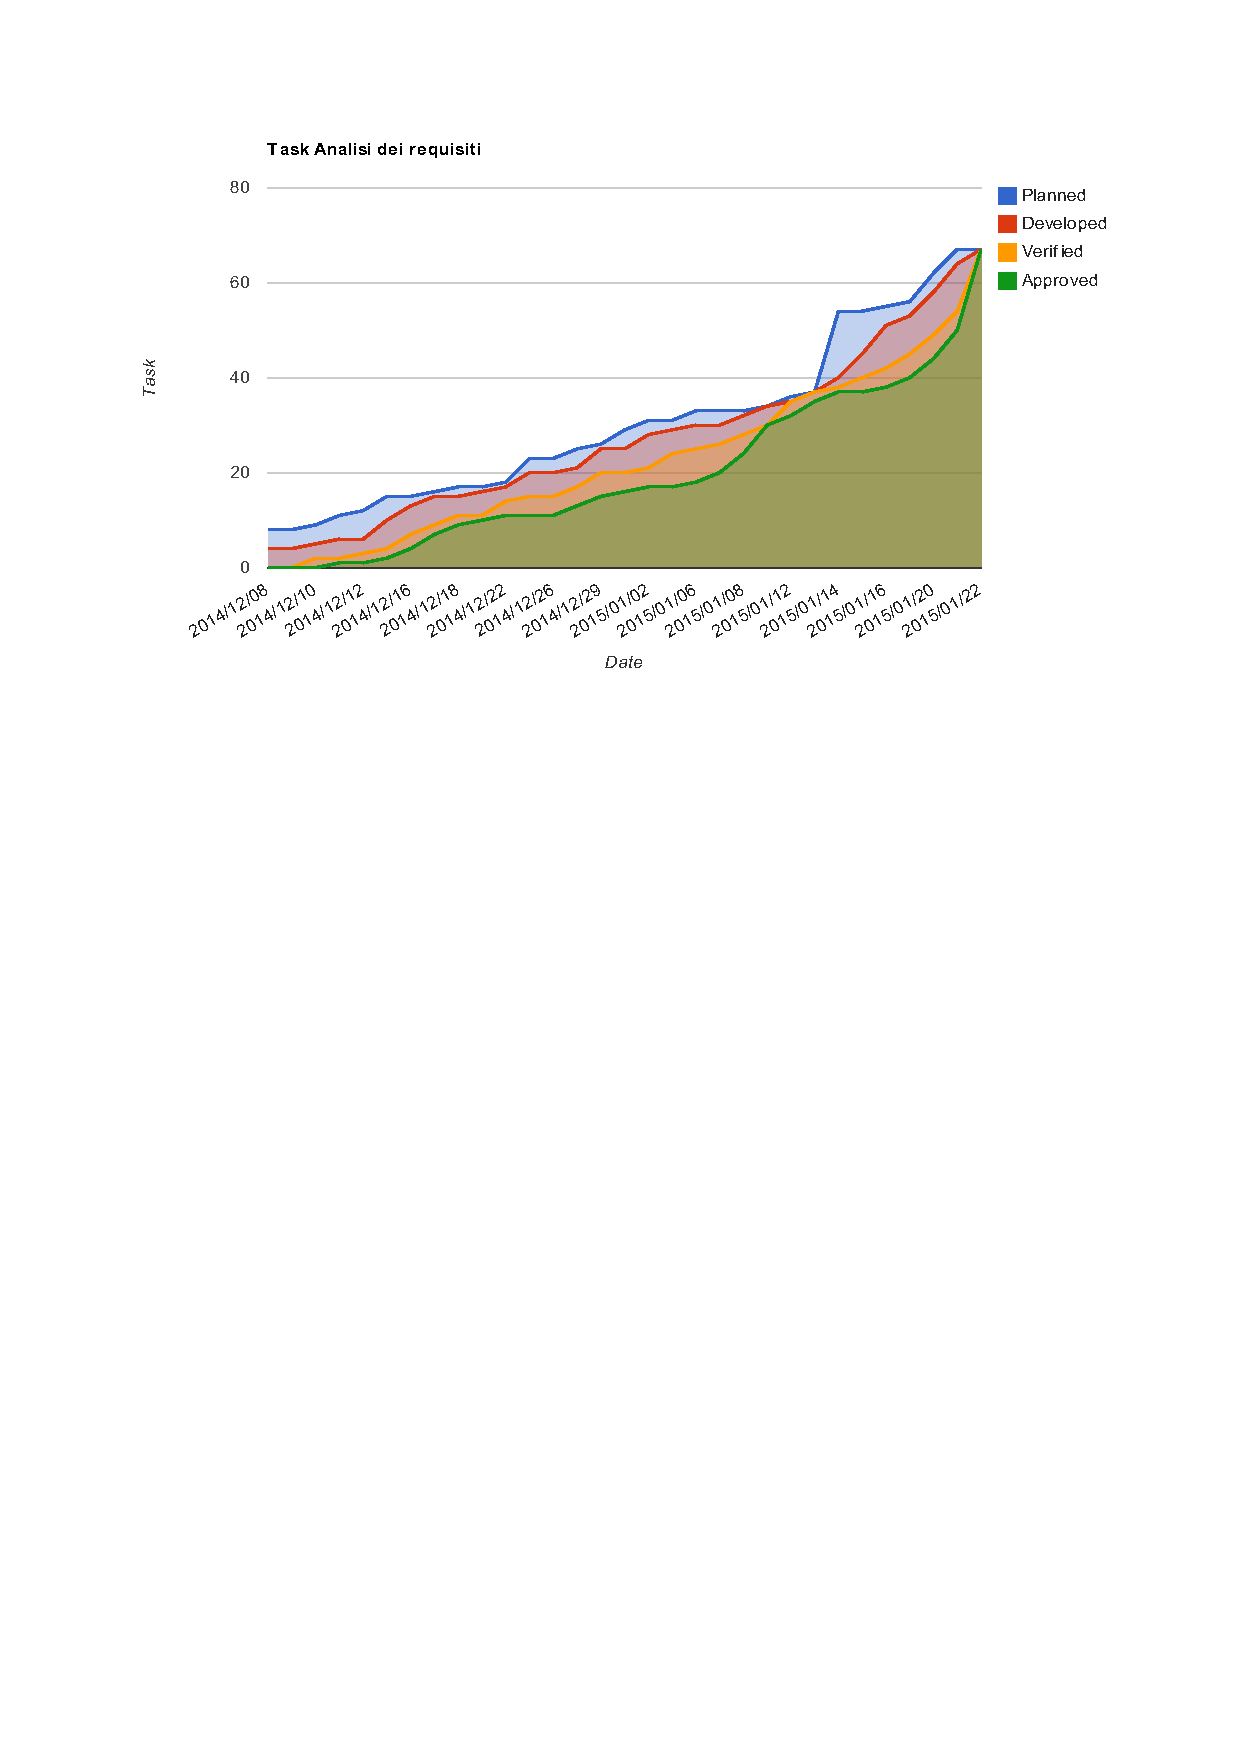
\includegraphics[scale=1]{images/Grafico_fase_2.pdf}}
				\caption{Grafico task Analisi dei requisiti}
				\label{fig:taskfase2}
			\end{figure}
	 	\subsubsection{Documenti}
	 	Vengono riportati i valori dell'indice di Gulpease relativi alla fase Analisi dei requisiti. Un documento va considerato accettabile solamente se rientra nelle metriche definite nella sezione.
		\begin{table}[!ht]
			\begin{center}
				\begin{tabularx}{0.9\textwidth}{|l|l|X|}
					\hline
					\textbf{Nome documento} & \textbf{Valore indice} & \textbf{Esito}\\
					\hline						
					\emph{Analisi dei Requisiti v1.0.0} & 56 & \textcolor{green}{Superato}\\
					\hline
					\emph{Glossario v1.0.0} & 50 & \textcolor{green}{Superato}\\
					\hline					
					\emph{Norme di Progetto v1.0.0} & 54 & \textcolor{green}{Superato}\\
					\hline					
					\emph{Piano di Progetto v1.0.0} & 55 & \textcolor{green}{Superato}\\
					\hline					
					\emph{Piano di Qualifica v1.0.0} & 55 & \textcolor{green}{Superato}\\
					\hline					
					\docNameVersionSdF & 48 & \textcolor{green}{Superato}\\
					\hline				
				\end{tabularx}
			\end{center}
			\caption{Risultati indice Gulpease - Analisi dei requisiti}
		\end{table}
		
	\subsection{Analisi di dettaglio}
		\subsubsection{Processi}
		Inizialmente sono presenti molti task già pianificati questo anche perché la  riunione del team è stata fatta nel periodo iniziale della fase. Grazie a tale accorgimento è stato possibile pianificare con anticipo i task e quindi dare maggiore libertà in termini di tempistiche a coloro che dovevano completarli,  approvarli e verificarli.  \\
		Nel grafico si può notare che c'è un notevole aumento dei task Verified e Approved tra il 2015/02/05 e il 2015/02/06, i motivo e che il \roleProjectManager \ ha fissato la data di consegna di tutte le parti della presentazione il 2015/02/06. Il gruppo di conseguenza, ha cercato di rispettare al meglio la consegna, questo ha fatto si che ci fossero le giuste tempistiche per le prove della presentazione nonché l'integrazione con tutte le parti. Si osserva in oltre che non sono stati completati tutti i task pianificati, il motivo è che tutti i membri del gruppo negli ultimi giorni si sono impegnati a perfezionare la presentazione tralasciando in parte il lavoro da svolgere. Il non completamento di tutti i task andrà perciò ad appesantire la fase successiva nella quale bisognerà integrare anche questi task a quelli della fase.
		\begin{figure}[htbp]
				\centering
				\centerline{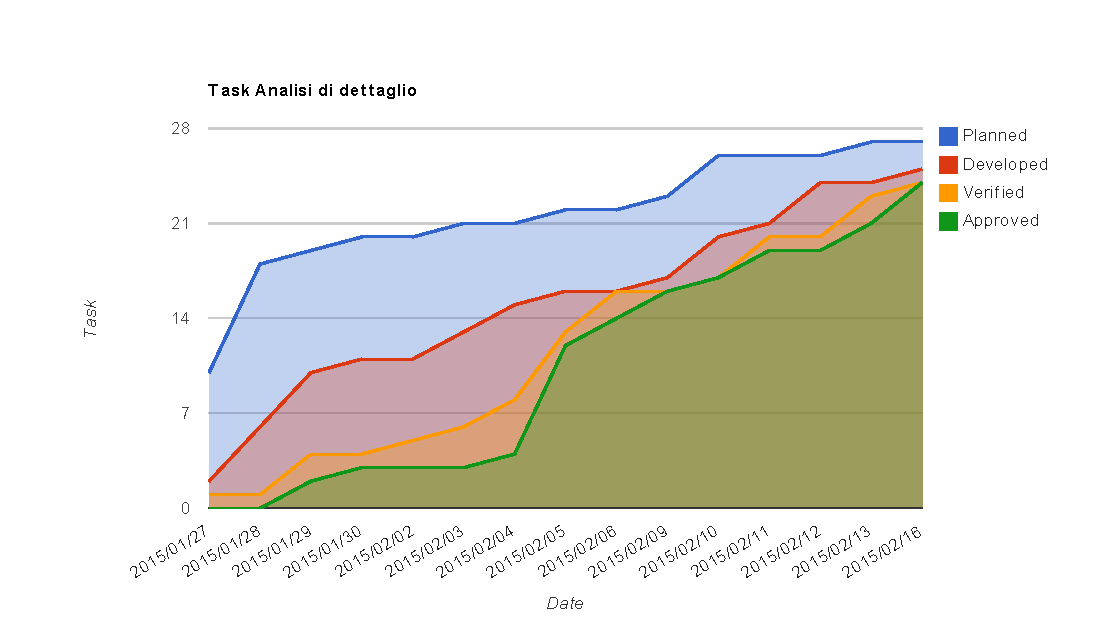
\includegraphics[scale=1]{images/Grafico_fase_3.pdf}}
				\caption{Grafico task Analisi di dettaglio}
				\label{fig:taskfase3}
			\end{figure}	
				
	 	\subsubsection{Documenti}
	 	Vengono riportati i valori dell'indice di Gulpease relativi alla fase Analisi di dettaglio. Un documento va considerato accettabile solamente se rientra nelle metriche definite nella sezione.
		\begin{table}[!ht]
			\begin{center}
				\begin{tabularx}{0.9\textwidth}{|l|l|X|}
					\hline
					\textbf{Nome documento} & \textbf{Valore indice} & \textbf{Esito}\\
					\hline						
					\emph{Analisi dei Requisiti v2.0.0} & 57 & \textcolor{green}{Superato}\\
					\hline
					\emph{Glossario v2.0.0} & 50 & \textcolor{green}{Superato}\\
					\hline					
					\emph{Norme di Progetto v2.0.0} & 55 & \textcolor{green}{Superato}\\
					\hline					
					\emph{Piano di Progetto v2.0.0} & 57 & \textcolor{green}{Superato}\\
					\hline					
					\emph{Piano di Qualifica v1.0.0} & 59 & \textcolor{green}{Superato}\\
					\hline					
					\docNameVersionSdF & 48 & \textcolor{green}{Superato}\\
					\hline				
				\end{tabularx}
			\end{center}
			\caption{Risultati indice Gulpease - Analisi di dettaglio}
		\end{table}
		
	\subsection{Progettazione architetturale}
		\subsubsection{Processi}
		Visto il successo riscontrato nella fase precedente si è deciso di rendere una best practice la volontà di fissare una riunione nel primo periodo della fase per pianificare il più possibile e aver successivamente più tempo per il completamento, la verifica e l'approvazione. Nonostante quest'accorgimento il gruppo ha sforato la data pianificata di chiusura della fase che era il 2015/03/23, per finire ad approvare gli ultimi task il 2015/03/30. Il ritardo è stato dato in parte dal fatto che i membri del gruppo si sono scontrati con un nuovo linguaggio, e con nuovi software, questi hanno avuto bisogno di un apprendimento, attraverso studio e incontri col proponente, che è durato più del panificato. Si è scelto di estendere il grafico fino alla data di effettiva approvazione dell'ultimo task per dar maggior visibilità al way of working.
		\begin{figure}[htbp]
				\centering
				\centerline{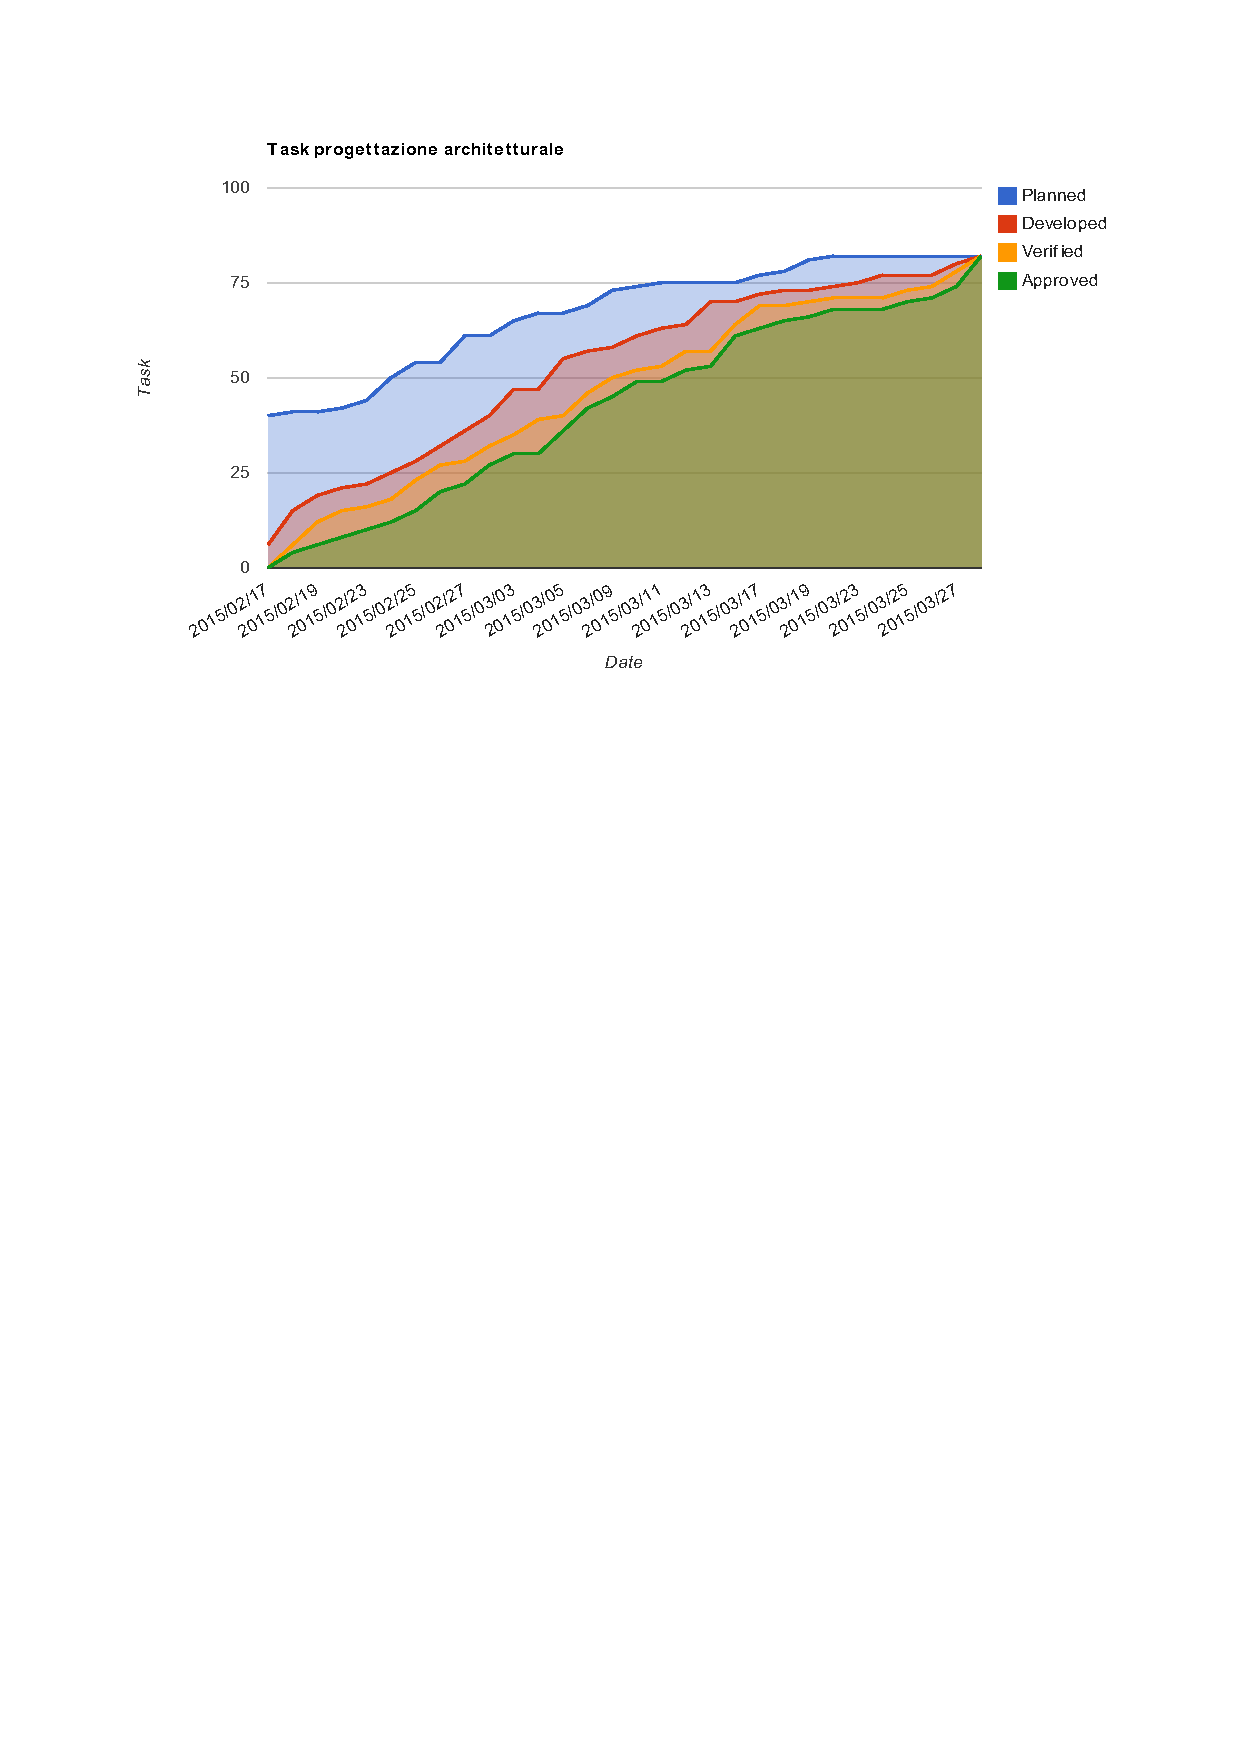
\includegraphics[scale=1]{images/Grafico_fase_4.pdf}}
				\caption{Grafico task Progettazione architetturale}
				\label{fig:taskfase4}
			\end{figure}
			
	 	\subsubsection{Documenti}	 	
	 	Vengono riportati i valori dell'indice di Gulpease relativi alla fase Progettazione architetturale. Un documento va considerato accettabile solamente se rientra nelle metriche definite nella sezione.
		\begin{table}[!ht]
			\begin{center}
				\begin{tabularx}{0.9\textwidth}{|l|l|X|}
					\hline
					\textbf{Nome documento} & \textbf{Valore indice} & \textbf{Esito}\\
					\hline						
					\docNameVersionAdR & 57 & \textcolor{green}{Superato}\\
					\hline
					\docNameVersionGlo & 51 & \textcolor{green}{Superato}\\
					\hline					
					\docNameVersionNdP & 55 & \textcolor{green}{Superato}\\
					\hline					
					\docNameVersionPdP & 57 & \textcolor{green}{Superato}\\
					\hline					
					\docNameVersionPdQ & 58 & \textcolor{green}{Superato}\\
					\hline					
					\docNameVersionSdF & 48 & \textcolor{green}{Superato}\\
					\hline	
					\docNameVersionST & 56 & \textcolor{green}{Superato}\\
					\hline			
				\end{tabularx}
			\end{center}
			\caption{Risultati indice Gulpease - Progettazione architetturale}
		\end{table}
		
	\subsection{Progettazione di dettaglio e codifica dei requisiti obbligatori}
		\subsubsection{Processi}
		La best practice usata nelle fasi precedenti è stata applicata anche qui. Nonostante questo tutti i task pianificati non sono stati completati entro la data di fine fase, 2015/05/08. Il ritardo è stato causato dalla pianificazione in difetto per quanto riguarda le ore di programmazione ed alcune rivisitazioni dei diagrammi delle classi completati in precedenza. I task che non sono stati \textit{Developed}, \textit{Verified}, \textit{Approved} andranno ad appesantire ulteriormente la fase successiva e chiederanno un impegno maggiore a tutto il gruppo per completarli entro la data fissata dal proponente.		
			\begin{figure}[htbp]
				\centering
				\centerline{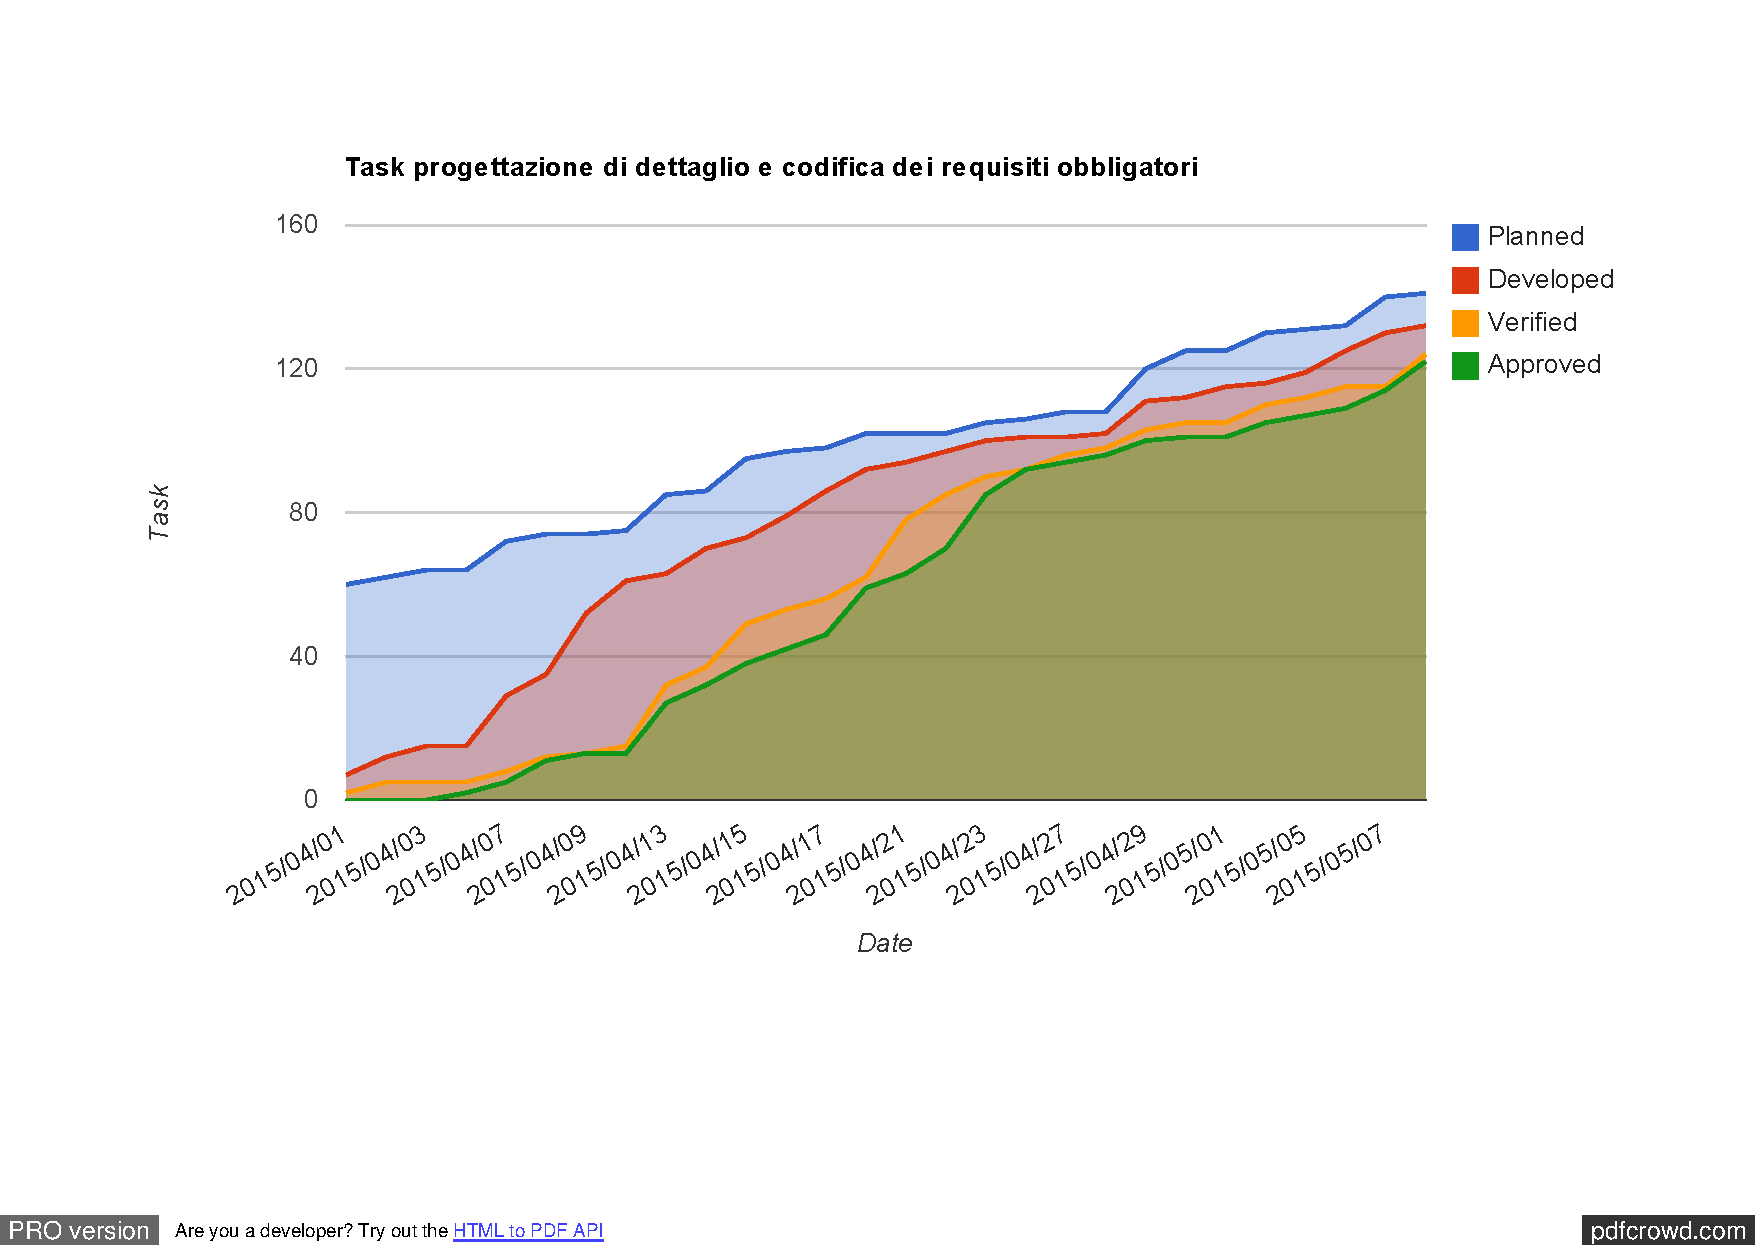
\includegraphics[scale=0.6]{images/Grafico_fase_5.pdf}}
				\caption{Grafico task Progettazione di dettaglio e codifica dei requisiti obbligatori}
				\label{fig:taskfase5}
			\end{figure}
			
	 	\subsubsection{Documenti}	 	
	 	Vengono riportati i valori dell'indice di Gulpease relativi alla fase Progettazione di dettaglio e codifica dei requisiti obbligatori. Un documento va considerato accettabile solamente se rientra nelle metriche definite nella sezione.
		\begin{table}[!ht]
			\begin{center}
				\begin{tabularx}{0.9\textwidth}{|l|l|X|}
					\hline
					\textbf{Nome documento} & \textbf{Valore indice} & \textbf{Esito}\\
					\hline						
					\docNameVersionAdR & ?? & \textcolor{green}{Superato}\\
					\hline
					\docNameVersionGlo & ?? & \textcolor{green}{Superato}\\
					\hline					
					\docNameVersionNdP & ?? & \textcolor{green}{Superato}\\
					\hline					
					\docNameVersionPdP & ?? & \textcolor{green}{Superato}\\
					\hline					
					\docNameVersionPdQ & ?? & \textcolor{green}{Superato}\\
					\hline					
					\docNameVersionSdF & ?? & \textcolor{green}{Superato}\\
					\hline	
					\docNameVersionST & ?? & \textcolor{green}{Superato}\\
					\hline			
				\end{tabularx}
			\end{center}
			\caption{Risultati indice Gulpease - Progettazione di dettaglio e codifica dei requisiti obbligatori}
		\end{table}
		
		\subsubsection{Progettazione}
		Viene riportata di seguito una tabella riassuntiva (tabella 10) che espone gli indici di instabilità per i componenti rilevati durante la progettazione. In questa tabella in oltre viene specificato come i componenti superano questo test, se in modo ottimale, scritta in \textcolor{green}{verde} o in modo accettabile \textcolor{yellow}{giallo}. Le componenti invece che non superano il test sono contrassegnate con la scritta \textit{Non Superato} in \textcolor{red}{rosso}. Per quanto riguarda le componenti che non hanno superato il test non si pianificano degli obbiettivi di miglioramento in quanto il non superamento è causato dalla natura e dalla funzionalità dei componenti stessi.
		\begin{center}

			\def\arraystretch{1.5}
			\bgroup
			\begin{longtable}{| p{8.5cm} | p{3.5cm} | p{3cm} |}
					\hline
					\textbf{Componente} & \textbf{Indice instabilità} & \textbf{Esito}\\
					\hline
					\texttt{src::client::model} & 0 & \textcolor{green}{Superato}\\
					\hline
					\texttt{src::client::model::data} & 0.75 & \textcolor{yellow}{Superato}\\
					\hline
					\texttt{src::client::model::services} & 0.33 & \textcolor{green}{Superato}\\
					\hline
					\texttt{src::client::view} & 0.5 & \textcolor{green}{Superato}\\ 
					\hline
					\texttt{src::client::view::public} & 0.5 & \textcolor{green}{Superato}\\
					\hline
					\texttt{src::client::view::user} & 0.33 & \textcolor{green}{Superato}\\
					\hline
					\texttt{src::client::view::admin} & 0.66 & \textcolor{green}{Superato}\\
					\hline
					\texttt{src::client::controller} &  0.75 & \textcolor{yellow}{Superato}\\
					\hline
					\texttt{src::client::controller::public} & 0.75 & \textcolor{yellow}{Superato}\\
					\hline
					\texttt{src::client::controller::user} & 0.75 & \textcolor{yellow}{Superato}\\
					\hline
					\texttt{src::client::controller::admin} & 0.75 & \textcolor{yellow}{Superato}\\
					\hline
					\texttt{src::server::db} & 0 & \textcolor{green}{Superato}\\
					\hline
					\texttt{src::server::db::raw\_data} & 0 & \textcolor{green}{Superato}\\ 
					\hline
					\texttt{src::server::db::raw\_data::fb} & 0.8 & \textcolor{yellow}{Superato}\\
					\hline
					\texttt{src::server::db::raw\_data::tw} & 0.75 & \textcolor{yellow}{Superato}\\
					\hline
					\texttt{src::server::db::raw\_data::ig} & 0.8 & \textcolor{yellow}{Superato}\\
					\hline
					\texttt{src::server::db::app\_data} & 0 & \textcolor{green}{Superato}\\
					\hline
					\texttt{src::server::db::app\_data::user} & 0.75 & \textcolor{yellow}{Superato}\\
					\hline
					\texttt{src::server::db::app\_data::recipe} & 0 & \textcolor{green}{Superato}\\
					\hline
					\texttt{src::server::processor} & 0.8 & \textcolor{yellow}{Superato}\\
					\hline
					\texttt{src::server::processor::commands} & 0.8 & \textcolor{yellow}{Superato}\\
					\hline
					\texttt{src::server::processor::commands::user} & 1 & \textcolor{red}{Non Superato}\\
					\hline
					\texttt{src::server::processor::commands::recipe} & 1 & \textcolor{red}{Non Superato}\\
					\hline
					\texttt{src::server::processor::commands::requests} & 1 & \textcolor{red}{Non Superato}\\
					\hline
					\texttt{src::server::processor::commands::social} & 1 & \textcolor{red}{Non Superato}\\
					\hline
					\texttt{src::server::miner} & 0.75 & \textcolor{yellow}{Superato}\\
					\hline
					\texttt{src::server::miner::fb} & 1 & \textcolor{red}{Non Superato}\\
					\hline
					\texttt{src::server::miner::tw} & 1 & \textcolor{red}{Non Superato}\\
					\hline
					\texttt{src::server::miner::ig} & 1 & \textcolor{red}{Non Superato}\\
					\hline
					\texttt{src::server::endpoints} & ?? & ??\\
					\hline
					\texttt{src::server::endpoints::api} & ?? & ??\\
					\hline
					\texttt{src::server::endpoints::api::public} & ?? & ??\\
					\hline
					\texttt{src::server::endpoints::api::private} & ?? & ??\\
					\hline
					\texttt{src::server::endpoints::resp} & ?? & ??\\
					\hline
					\texttt{src::server::endpoints::resp::public} & ?? & ??\\
					\hline
					\texttt{src::server::endpoints::resp::public::fb} & ?? & ??\\
					\hline
					\texttt{src::server::endpoints::resp::public::tw} & ?? & ??\\
					\hline
					\texttt{src::server::endpoints::resp::public::ig} & ?? & ??\\
					\hline
					\texttt{src::server::endpoints::resp::private} & ?? & ??\\
					\hline
					\caption{Tracciamento test di sistema - requisiti}
				\end{longtable}
				\egroup
			\end{center}		
			
		\subsubsection{Metriche codice}
			Questa sezione traccia i risultati ricavati applicando le metriche relative al codice descritte nella sezione 2.8.3 di questo documento. Si è scelto di mantenere una separazione tra client e backend, in alcune metriche inoltre si specifica sia la media di tale indice che il valore massimo. Segue ogni metrica, una breve descrizione dove si specifica se il test è stato superato o in caso negativo il motivo presunto per cui non lo è.\\
			\begin{description}
				\item \textbf{Indice di copertura:}				
				\begin{itemize}
						\item Backend:
							\begin{itemize}
								\item medio: ??
								\item massimo: ??
							\end{itemize}
						\item Client:
							\begin{itemize}
								\item medio: ??
								\item massimo: ??
							\end{itemize}
					\end{itemize}
				
				\item \textbf{Complessità ciclomatica:}
					\begin{itemize}
						\item Backend:
							\begin{itemize}
								\item medio: ??
								\item massimo: ??
							\end{itemize}
						\item Client:
							\begin{itemize}
								\item medio: ??
								\item massimo: ??
							\end{itemize}
					\end{itemize}
						
				\item \textbf{Numero di parametri per metodo:}
					\begin{itemize}
						\item Backend:
							\begin{itemize}
								\item medio: ??
								\item massimo: ??
							\end{itemize}
						\item Client:
							\begin{itemize}
								\item medio: ??
								\item massimo: ??
							\end{itemize}
					\end{itemize}
					
				\item \textbf{Linee di codice per linee di commento:}
					\begin{itemize}
						\item Backend:
							\begin{itemize}
								\item medio: ??
								\item massimo: ??
							\end{itemize}
						\item Client:
							\begin{itemize}
								\item medio: ??
								\item massimo: ??
							\end{itemize}
					\end{itemize}
							
				\item \textbf{Numero di livelli di annidamento:}
					\begin{itemize}
						\item Backend:
							\begin{itemize}
								\item medio: ??
								\item massimo: ??
							\end{itemize}
						\item Client:
							\begin{itemize}
								\item medio: ??
								\item massimo: ??
							\end{itemize}
					\end{itemize}
					
				\item \textbf{Logical SLOC:}
					\begin{itemize}
						\item Backend:
						\item Client:
					\end{itemize}
					
	\subsection{Progettazione di dettaglio e codifica dei requisiti desiderabili}
		\subsubsection{Processi}
		Questa fase è stata appesantita dai ritardi accumolati nella fase precedente. Per questo motivo nel grafico non sono stati riportati i task pianificati nella fase antecedente, mentre i task che non erano stati \textit{Developed}, \textit{Verified}, \textit{Approved}, sono stati completati qui, togliendo tempo ai task pianificati in questa fase. Il risultato è che i task per i requisiti obbligatori sono stati completati, mentre parte di quelli per i requisiti desiderabili non sono stati sviluppati. Questo andrà ad aumentare il lavoro della fase successiva, con la possibilità di non terminare i requisiti opzionali.
			\begin{figure}[htbp]
				\centering
				\centerline{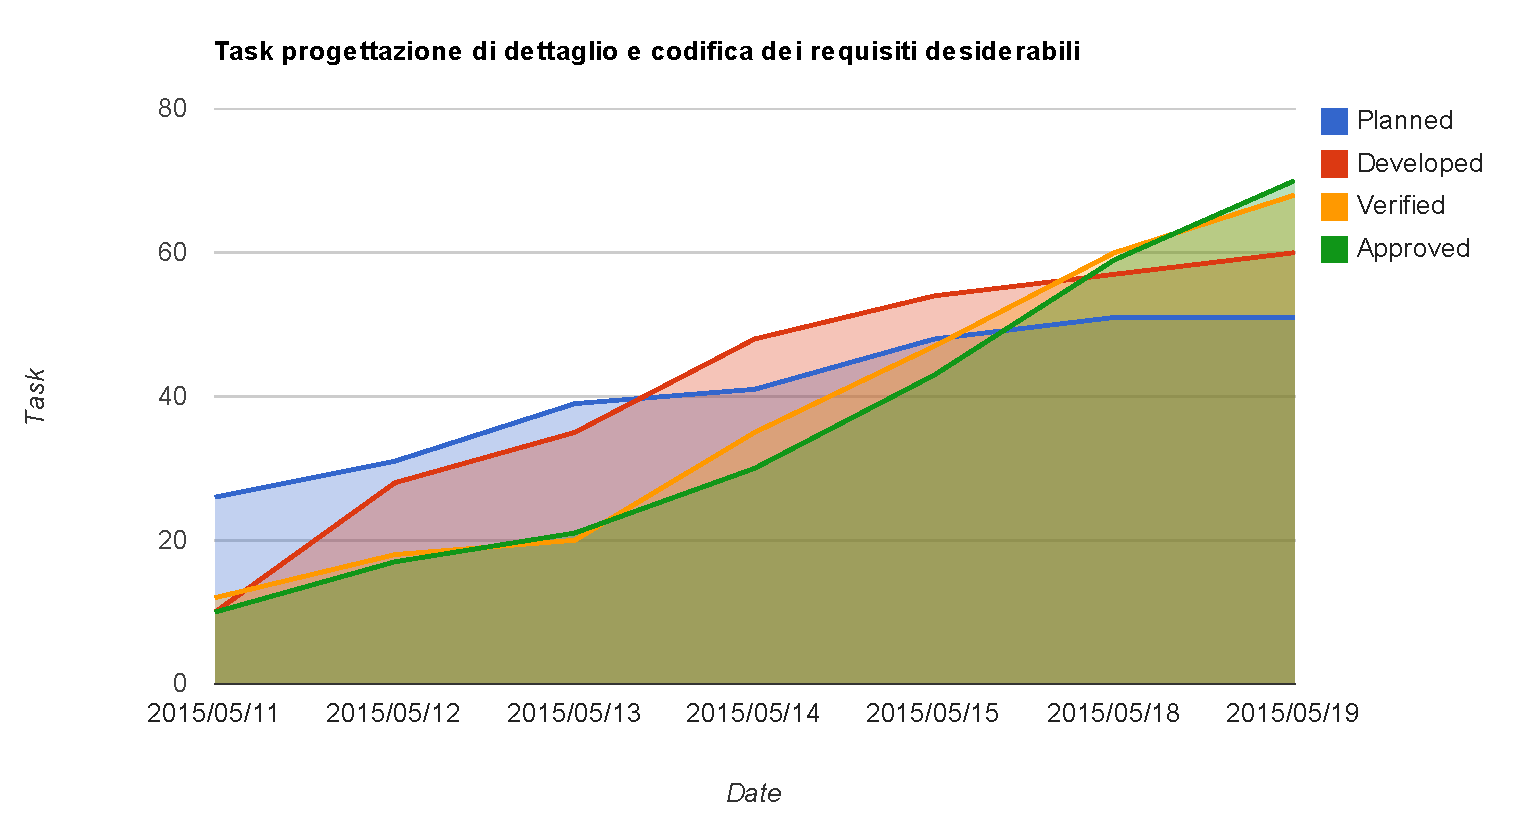
\includegraphics[scale=0.6]{images/Grafico_fase_6.pdf}}
				\caption{Grafico task Progettazione di dettaglio e codifica dei requisiti desiderabili}
				\label{fig:taskfase6}
			\end{figure}
			
	 	\subsubsection{Documenti}	 	
	 	Vengono riportati i valori dell'indice di Gulpease relativi alla fase Progettazione di dettaglio e codifica dei requisiti desiderabili. Un documento va considerato accettabile solamente se rientra nelle metriche definite nella sezione.
		\begin{table}[!ht]
			\begin{center}
				\begin{tabularx}{0.9\textwidth}{|l|l|X|}
					\hline
					\textbf{Nome documento} & \textbf{Valore indice} & \textbf{Esito}\\
					\hline						
					\docNameVersionAdR & ?? & \textcolor{green}{Superato}\\
					\hline
					\docNameVersionGlo & ?? & \textcolor{green}{Superato}\\
					\hline					
					\docNameVersionNdP & ?? & \textcolor{green}{Superato}\\
					\hline					
					\docNameVersionPdP & ?? & \textcolor{green}{Superato}\\
					\hline					
					\docNameVersionPdQ & ?? & \textcolor{green}{Superato}\\
					\hline					
					\docNameVersionSdF & ?? & \textcolor{green}{Superato}\\
					\hline	
					\docNameVersionST & ?? & \textcolor{green}{Superato}\\
					\hline			
				\end{tabularx}
			\end{center}
			\caption{Risultati indice Gulpease - Progettazione di dettaglio e codifica dei requisiti desiderabili}
		\end{table}
	
\pagebreak